\documentclass[conference]{IEEEtran}
\IEEEoverridecommandlockouts
\usepackage[indonesian]{babel}
\usepackage{cite}
\usepackage{amsmath,amssymb,amsfonts}
\usepackage{graphicx}
\usepackage{textcomp}
\usepackage{xcolor}
\usepackage{booktabs}
\usepackage{url}
\graphicspath{{figures/}}
\addto\captionsindonesian{%
  \renewcommand{\abstractname}{Abstrak}%
  \renewcommand{\refname}{Referensi}%
}
\renewcommand{\IEEEkeywordsname}{Kata Kunci}

\begin{document}

\title{Jejak Budaya dalam Nama: Klasifikasi, Klastering, dan Generasi Nama Desa di Indonesia Berbasis N-gram Karakter}

\author{
\IEEEauthorblockN{Dina Hamala Nur Rosyidah (L0124010), Fadhil Rusadi (L0124013), Firizqi Aditya Mulya (L0124016),\\
Muhammad Ihza Dzikrullah (L0124024), Andre Saputra (L0124038)}
\IEEEauthorblockA{\textit{Program Studi Informatika, Fakultas Teknologi Informasi dan Sains Data} \\
\textit{Universitas Sebelas Maret}, Surakarta, Indonesia}
}

\maketitle

\begin{abstract}
Nama desa di Indonesia menyimpan jejak bahasa dan budaya daerahnya, misalnya awalan ``Ci-'' di tanah Sunda atau akhiran ``-rejo'' di Jawa. Penelitian ini mengukur seberapa banyak informasi tersebut dapat diekstraksi dari susunan huruf saja, memakai 83.758 nama desa dan kelurahan dari kode wilayah Kepmendagri Tahun 2025. Nama direpresentasikan dengan TF-IDF n-gram karakter, lalu dianalisis dengan tiga pendekatan. Pertama, klasifikasi provinsi (38 kelas) dan wilayah besar (7 kelas) dengan Naive Bayes, Logistic Regression, dan SVM, memakai pembagian data per nama unik untuk mencegah kebocoran. Model mencapai akurasi sekitar 40\% untuk provinsi (tebakan acak 2,6\%) dan 65\% sampai 68\% untuk wilayah, dengan akurasi top-3 sekitar 90\%. Kedua, klastering 514 kabupaten tanpa label dengan K-Means dan Ward, yang memisahkan wilayah Sunda dari Jawa serta Aceh pesisir dari dataran tinggi Gayo, dengan Adjusted Rand Index 0,42 sampai 0,46 terhadap pembagian wilayah resmi. Ketiga, generator nama berbasis rantai Markov karakter yang 71,7\% hasilnya ditebak classifier sesuai wilayah asalnya. Analisis kesalahan juga menemukan jejak program kolonisasi dan transmigrasi: desa di Lampung paling sering ditebak berasal dari Jawa, tertinggi di Kota Metro (45,5\%). Seluruh model disajikan dalam dasbor interaktif berbasis Streamlit.
\end{abstract}

\begin{IEEEkeywords}
nama desa, toponimi, n-gram karakter, klasifikasi teks, klastering, rantai Markov, transmigrasi
\end{IEEEkeywords}

\section{Pendahuluan}

Indonesia memiliki lebih dari 83 ribu desa dan kelurahan yang tersebar di 38 provinsi. Nama-nama tersebut tidak dibuat secara acak. Banyak nama desa di Jawa Barat diawali ``Ci-'' (dari kata Sunda \textit{cai}, air), banyak nama di Jawa Tengah dan Jawa Timur berakhiran ``-rejo'' atau ``-mulyo'', sementara nama di Sulawesi Selatan sering memakai konsonan ganda seperti ``Bonto'' dan ``Tamalatea''. Dengan kata lain, sebuah nama desa membawa sidik jari bahasa daerah tempat ia berada.

Pertanyaan yang diajukan penelitian ini bukan ``di mana letak desa X'', karena jawaban itu cukup dicari di basis data atau mesin pencari. Pertanyaannya adalah \textit{informasi budaya apa yang tersimpan dalam puluhan ribu nama desa Indonesia, dan seberapa banyak yang dapat diukur}. Model pembelajaran mesin dipakai sebagai alat untuk membedah pola tersebut. Pendekatan ini juga memiliki kegunaan praktis: model dapat menebak asal nama yang tidak ada di basis data (misalnya nama dusun atau nama desa lama di arsip), dapat menandai desa yang namanya sangat tidak cocok dengan provinsinya sebagai kandidat kesalahan kode wilayah, dan dapat memperlihatkan jejak sejarah sosial seperti transmigrasi.

Penelitian ini menjawab lima pertanyaan:
\begin{enumerate}
\item Seberapa akurat nama desa saja dapat menebak provinsi dan wilayah besar?
\item Potongan huruf apa yang paling khas untuk setiap daerah?
\item Tanpa label, apakah kabupaten mengelompok membentuk wilayah budaya berdasarkan kemiripan nama desanya?
\item Apakah kesalahan model menyimpan pola yang bermakna, misalnya jejak transmigrasi?
\item Apakah pola nama per daerah cukup kuat sehingga dapat ditiru untuk mengarang nama baru?
\end{enumerate}

Proyek ini dikerjakan mengikuti tujuh tahap \textit{Team-Based Project}: perumusan masalah, pengumpulan data, \textit{preprocessing}, pemodelan, evaluasi, purwarupa, dan presentasi. Bagian II membahas penelitian terkait, Bagian III menjelaskan data dan metode, Bagian IV menyajikan hasil dan pembahasan, dan Bagian V berisi kesimpulan serta saran.

\section{Penelitian Terkait}

Menebak asal dari sebuah nama telah diteliti pada nama orang. Ambekar dkk.\ \cite{ambekar2009} membangun pengklasifikasi etnis dari nama memakai data Wikipedia dan model urutan karakter, lalu menerapkannya pada puluhan juta nama di korpus berita. Ye dkk.\ \cite{ye2017} mengembangkan NamePrism yang mengklasifikasikan kewarganegaraan ke 39 kelompok memakai \textit{name embedding}. Kedua penelitian menunjukkan bahwa susunan huruf sebuah nama membawa sinyal asal-usul yang kuat.

Pada nama tempat (toponim), Fize dkk.\ \cite{fize2021} memakai \textit{embedding} n-gram karakter untuk \textit{geocoding} toponim, dengan alasan bahwa n-gram karakter efektif untuk teks yang mengandung variasi ejaan dan kata baru. Penggunaan n-gram karakter untuk kategorisasi teks sendiri sudah lama dikenal sejak Cavnar dan Trenkle \cite{cavnar1994}.

Di Indonesia, penelitian yang paling dekat adalah identifikasi bahasa daerah dari kalimat. Sujaini dan Putra \cite{sujaini2024} membandingkan beberapa algoritma, termasuk Naive Bayes dan KNN, dengan fitur n-gram untuk bahasa-bahasa daerah Indonesia. Winata dkk.\ \cite{winata2023} menyusun NusaX, korpus paralel untuk 10 bahasa daerah Indonesia. Penelitian-penelitian tersebut bekerja pada kalimat utuh, sedangkan penelitian ini bekerja pada nama tempat yang hanya terdiri dari satu sampai beberapa kata. Sejauh penelusuran penulis, belum ditemukan studi yang mengklasifikasikan atau mengklaster nama desa di Indonesia.

Untuk menafsirkan hasil, penelitian ini juga merujuk sejarah kolonisasi di Lampung. Program kolonisasi pemerintah Hindia Belanda dimulai di Gedong Tataan, Lampung, pada tahun 1905 dengan memindahkan penduduk dari Jawa \cite{sudarno2018}. Program ini kemudian dilanjutkan sebagai transmigrasi setelah kemerdekaan.

\section{Metodologi}

\subsection{Pengumpulan Data}

Data berasal dari kode dan nama wilayah administrasi sesuai Keputusan Menteri Dalam Negeri No.\ 300.2.2-2138 Tahun 2025 \cite{kepmendagri2025}, yang diambil dari repositori terbuka \texttt{cahyadsn/wilayah} \cite{cahyadsn} dalam format SQL. Data berisi 38 provinsi, 514 kabupaten/kota, 7.285 kecamatan, dan 83.762 desa/kelurahan (75.252 desa, 8.496 kelurahan, dan 14 desa adat). Repositori yang sama menyediakan poligon batas provinsi dan kabupaten, yang diubah ke format GeoJSON untuk pemetaan. Setiap provinsi juga dipetakan ke salah satu dari tujuh wilayah besar: Sumatera, Jawa, Bali dan Nusa Tenggara, Kalimantan, Sulawesi, Maluku, dan Papua.

\subsection{Preprocessing}

Prinsip pembersihan adalah membuang unsur administratif dan mempertahankan unsur yang membawa petunjuk budaya. Aturan diputuskan setelah memeriksa data:
\begin{itemize}
\item Nama diubah ke huruf kecil dan spasi dirapikan.
\item Awalan ``Desa Adat'' dibuang. Kata khas daerah di awal nama seperti \textit{gampong} (Aceh), \textit{huta} (Batak), \textit{pekon} (Lampung), dan \textit{lembang} (Toraja) justru dipertahankan.
\item Penanda pemekaran dibuang: angka romawi yang berdiri sendiri (sekitar 1.270 nama) dan potongan yang mengandung angka.
\item Singkatan di Aceh diperluas (``Mns.'' menjadi \textit{meunasah}, ``Tgk.'' menjadi \textit{teungku}), dan kata yang menempel dipisahkan.
\item Tanda baca dibuang, kecuali tanda petik (misalnya \textit{kandua\textquotesingle}) dan tanda hubung (misalnya \textit{sigurung-gurung}).
\item Empat nama berupa singkatan huruf kapital (misalnya ``OP'' dan ``MKCM'') tidak dipakai.
\end{itemize}
Hasilnya adalah 83.758 baris dengan 62.769 nama bersih unik dan tanpa nilai kosong.

\subsection{Representasi Fitur}

Setiap nama diubah menjadi vektor TF-IDF \cite{salton1988} dari n-gram karakter dengan panjang 2 sampai 4. N-gram diambil per kata dengan penanda batas kata, sehingga model dapat membedakan awalan (misalnya ``\_ci'', kata yang diawali ``ci'') dari akhiran (misalnya ``rejo\_''). Bobot fitur $t$ pada nama $d$ adalah
\begin{equation}
w_{t,d} = \left(1 + \ln \mathrm{tf}_{t,d}\right) \cdot \left(\ln \frac{1 + N}{1 + \mathrm{df}_t} + 1\right),
\end{equation}
dengan $\mathrm{tf}_{t,d}$ frekuensi $t$ pada $d$, $N$ jumlah nama latih, dan $\mathrm{df}_t$ jumlah nama yang mengandung $t$. Vektor setiap nama kemudian dinormalisasi dengan norma L2. Hanya n-gram yang muncul di minimal dua nama yang dipakai, sehingga diperoleh sekitar 25 ribu fitur.

\subsection{Klasifikasi}

Tiga model dibandingkan untuk dua target, yaitu provinsi (38 kelas) dan wilayah besar (7 kelas): Multinomial Naive Bayes \cite{mccallum1998} sebagai \textit{baseline} klasik untuk teks, Logistic Regression yang koefisiennya dapat ditafsirkan dan menghasilkan probabilitas, serta SVM linear \cite{cortes1995,fan2008} yang umumnya kuat untuk fitur teks berdimensi tinggi. Karena jumlah desa per provinsi sangat timpang, Logistic Regression dan SVM memakai bobot kelas seimbang. Semua model diimplementasikan dengan scikit-learn \cite{pedregosa2011}.

Banyak nama dipakai oleh lebih dari satu desa, misalnya ``Sidomulyo'' yang muncul di 98 desa. Jika data dibagi acak per baris, nama yang sama dapat muncul di data latih dan data uji sekaligus sehingga akurasi menjadi semu. Ini adalah bentuk kebocoran data \cite{kaufman2012}. Karena itu data dibagi \textit{per nama unik}: 80\% nama untuk latih (67.374 baris) dan 20\% untuk uji (16.384 baris), dan dipastikan tidak ada nama yang muncul di keduanya.

Metrik evaluasi adalah akurasi, macro-F1 (rata-rata F1 semua kelas dengan bobot sama sehingga provinsi kecil dihitung adil), dan akurasi top-3 (persentase jawaban benar yang berada di tiga tebakan teratas). Sebagai pembanding dipakai model yang selalu menebak kelas terbanyak.

\subsection{Analisis Kesalahan}

Model akhir dilatih ulang dengan seluruh data, sehingga tidak dapat dipakai untuk menilai kesalahan pada data yang sama. Untuk analisis kesalahan dipakai prediksi \textit{out-of-fold}: data dibagi lima bagian per nama unik, dan setiap bagian ditebak oleh model yang dilatih dari empat bagian lainnya. Dengan begitu setiap desa memperoleh tebakan dari model yang belum pernah melihat namanya. Dari prediksi ini dihitung \textit{confusion matrix}, persentase desa di luar Jawa yang ditebak sebagai provinsi di Jawa, dan daftar desa yang ditebak sangat yakin ($p \geq 0{,}9$) ke wilayah besar yang berbeda dari labelnya.

\subsection{Klastering}

Setiap kabupaten diwakili oleh rata-rata vektor TF-IDF semua nama desanya, lalu dinormalisasi. Dimensi diperkecil menjadi 20 komponen dengan TruncatedSVD \cite{halko2011}. Dua metode dibandingkan: K-Means \cite{lloyd1982} dengan inisialisasi k-means++ \cite{arthur2007}, dan \textit{agglomerative clustering} dengan kriteria Ward \cite{ward1963}. Jumlah klaster $k = 2$ sampai 15 dinilai dengan \textit{silhouette score} \cite{rousseeuw1987}, yang tidak memakai label. Setelah itu, kecocokan klaster dengan provinsi dan wilayah resmi diukur dengan Adjusted Rand Index (ARI) \cite{hubert1985}, yang bernilai 0 untuk pengelompokan acak dan 1 untuk pengelompokan identik.

\subsection{Generator Nama}

Untuk setiap wilayah besar dibangun rantai Markov karakter \cite{shannon1948} berorde $n$: peluang huruf berikutnya bergantung pada $n$ huruf sebelumnya,
\begin{equation}
P(c_i \mid c_{i-n}, \ldots, c_{i-1}) = \frac{\mathrm{count}(c_{i-n} \ldots c_{i-1} c_i)}{\mathrm{count}(c_{i-n} \ldots c_{i-1})}.
\end{equation}
Nama dibangun huruf demi huruf sampai muncul tanda akhir, dan nama yang ternyata sudah ada di data dibuang. Kualitas generator diukur dengan dua cara: persentase nama yang benar-benar baru, dan persentase nama baru yang ditebak oleh classifier wilayah sesuai wilayah asal generatornya.

\subsection{Purwarupa}

Seluruh hasil disajikan dalam dasbor web berbasis Streamlit \cite{streamlit} yang terdiri dari empat halaman: tebak nama desa, peta klaster, fakta menarik, serta generator dan kuis.

\section{Hasil dan Pembahasan}

\begin{figure*}[!t]
\centering
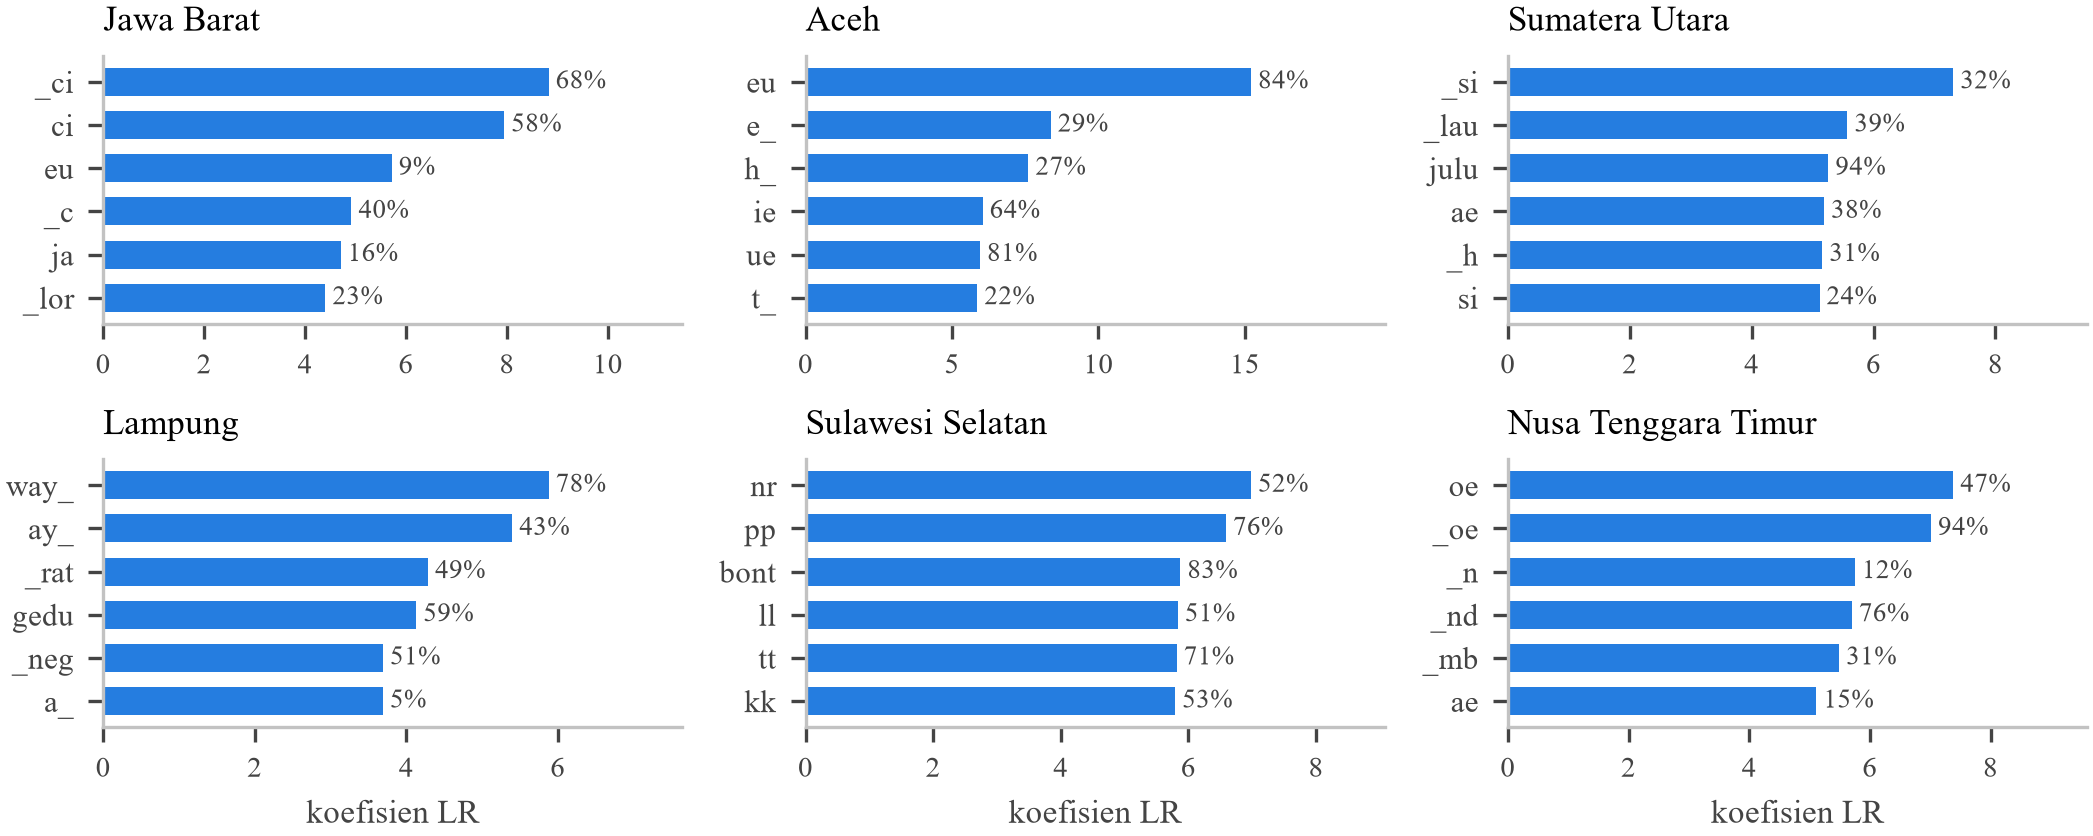
\includegraphics[width=\textwidth]{laporan_ngram.png}
\caption{N-gram paling khas untuk enam provinsi. Panjang batang adalah koefisien Logistic Regression; angka di ujung batang adalah persentase desa yang mengandung n-gram tersebut dan berada di provinsi itu. Tanda \_ menandai batas kata.}
\label{fig:ngram}
\end{figure*}

\subsection{Eksplorasi Data}

\begin{table}[!t]
\caption{Tiga kata pertama paling umum per wilayah (persen desa)}
\label{tab:katapertama}
\centering
\begin{tabular}{ll}
\toprule
Wilayah & Kata pertama \\
\midrule
Sumatera & tanjung (2,9), sungai (1,5), suka (1,1) \\
Jawa & karanganyar (0,3), sidomulyo (0,2), mekarsari (0,2) \\
Bali-Nusa Tenggara & golo (1,5), compang (0,6), watu (0,5) \\
Kalimantan & sungai (5,0), tumbang (2,6), tanjung (2,2) \\
Sulawesi & bonto (0,6), batu (0,4), buntu (0,3) \\
Maluku & kampung (0,5), batu (0,5), air (0,4) \\
Papua & muara (0,2), pasir (0,1), bumi (0,1) \\
\bottomrule
\end{tabular}
\end{table}

Jumlah desa sangat timpang: Jawa Tengah (8.563) memiliki 32 kali lipat jumlah desa DKI Jakarta (267), dan Sumatera bersama Jawa mencakup sekitar 61\% data. Nama desa umumnya pendek, dengan median 9 huruf, dan 63,8\% hanya terdiri dari satu kata. Dari 62.769 nama unik, 4.250 dipakai di lebih dari satu provinsi; yang paling tersebar adalah nama generik berbahasa Indonesia seperti ``Kampung Baru'' (24 provinsi) dan ``Mekar Jaya'' (18 provinsi).

Kata pertama nama desa sudah memperlihatkan ciri wilayah (Tabel~\ref{tab:katapertama}): \textit{sungai}, \textit{tumbang}, dan \textit{nanga} di Kalimantan, \textit{tanjung} dan \textit{blang} di Sumatera, \textit{bonto} di Sulawesi, serta \textit{golo} di Nusa Tenggara. Di Jawa polanya berbeda: kata pertama yang paling sering hanya mencakup 0,3\% desa, karena nama Jawa umumnya berupa satu kata gabungan seperti ``Karanganyar'' sehingga ciri khasnya berada di dalam kata.

\subsection{Klasifikasi}

Tabel~\ref{tab:klasifikasi} menunjukkan bahwa ketiga model jauh melampaui pembanding. Untuk provinsi, akurasi sekitar 40\%, atau sekitar 15 kali lipat tebakan acak (2,6\%), dan provinsi yang benar berada di tiga tebakan teratas pada sekitar 65\% kasus. Untuk wilayah besar, akurasi mencapai 65\% sampai 68\% dengan top-3 sekitar 90\%. Perbedaan antarmodel kecil: Naive Bayes unggul di akurasi provinsi, Logistic Regression di macro-F1 provinsi, dan SVM di target wilayah.

Logistic Regression dipilih sebagai model akhir untuk kedua target karena selisih macro-F1-nya dengan model terbaik kurang dari 0,02, sementara hanya model ini yang sekaligus menghasilkan probabilitas (dibutuhkan dasbor) dan koefisien per kelas yang dapat ditafsirkan (dibutuhkan analisis n-gram khas).

\begin{table}[!t]
\caption{Hasil klasifikasi pada data uji (dibagi per nama unik)}
\label{tab:klasifikasi}
\centering
\begin{tabular}{llccc}
\toprule
Target & Model & Akurasi & Macro-F1 & Top-3 \\
\midrule
Provinsi & Kelas terbanyak & 0,100 & 0,005 & - \\
 & Naive Bayes & \textbf{0,419} & 0,304 & \textbf{0,648} \\
 & Logistic Regression & 0,401 & \textbf{0,330} & 0,642 \\
 & SVM linear & 0,402 & 0,328 & 0,620 \\
\midrule
Wilayah & Kelas terbanyak & 0,307 & 0,067 & - \\
 & Naive Bayes & 0,654 & 0,541 & \textbf{0,899} \\
 & Logistic Regression & 0,651 & 0,557 & 0,892 \\
 & SVM linear & \textbf{0,678} & \textbf{0,571} & 0,895 \\
\bottomrule
\end{tabular}
\end{table}

\subsection{N-gram Paling Khas}

\begin{figure}[!t]
\centering
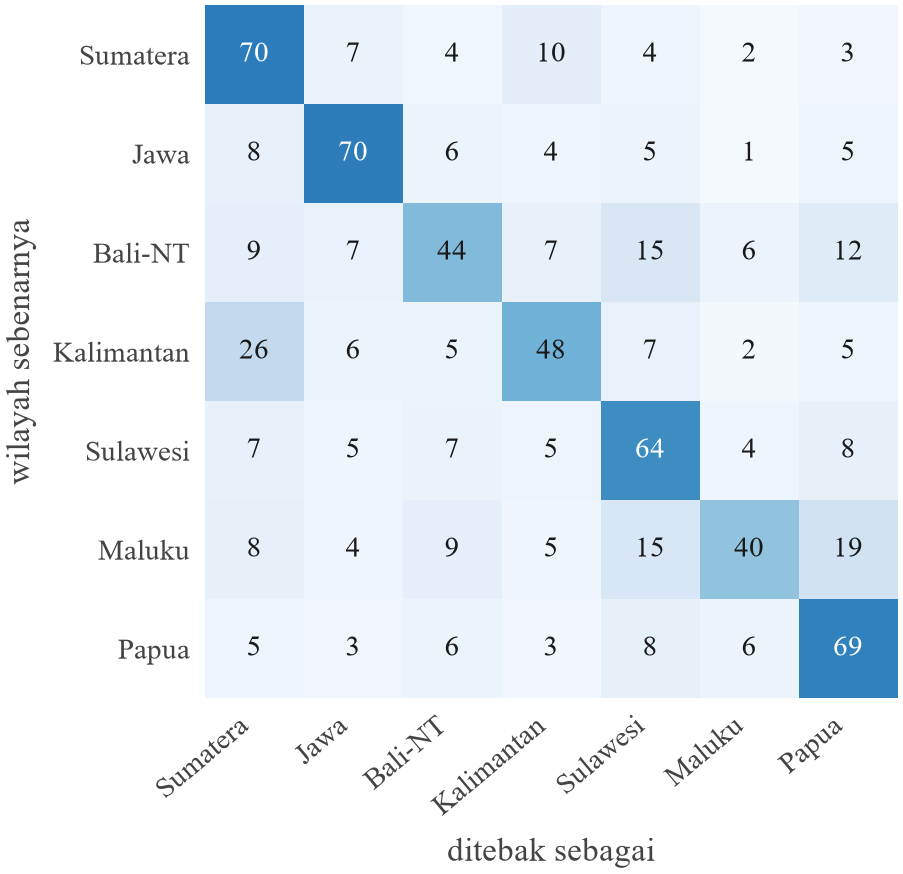
\includegraphics[width=0.92\columnwidth]{laporan_confusion.png}
\caption{\textit{Confusion matrix} wilayah besar dari prediksi \textit{out-of-fold}, dalam persen per baris.}
\label{fig:confusion}
\end{figure}

\begin{figure*}[!t]
\centering
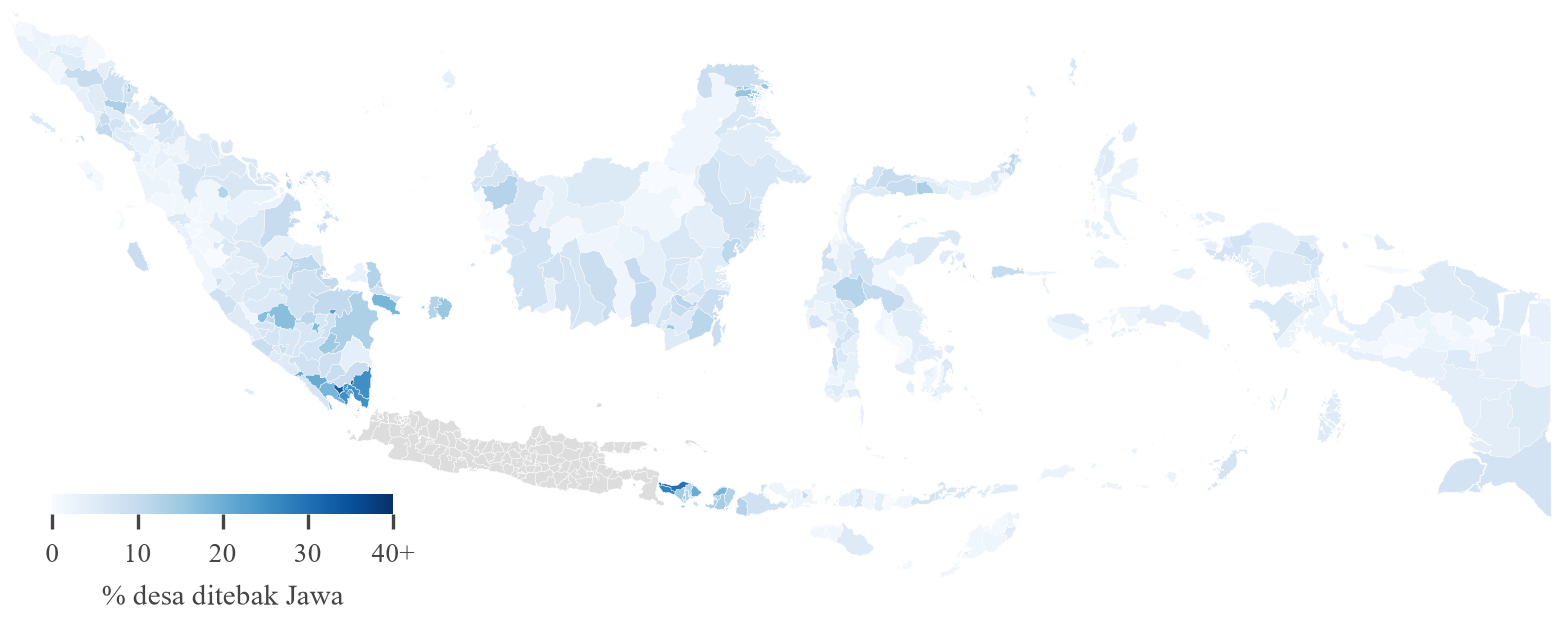
\includegraphics[width=\textwidth]{laporan_jejak_jawa.png}
\caption{Persentase desa di setiap kabupaten luar Jawa yang ditebak sebagai provinsi di Jawa (prediksi \textit{out-of-fold}). Pulau Jawa digambar abu-abu karena tidak dihitung. Warna tergelap berada di Lampung dan Bali.}
\label{fig:jejak}
\end{figure*}

Koefisien Logistic Regression memperlihatkan n-gram yang paling mendorong tebakan ke setiap provinsi; enam di antaranya ditampilkan pada Gbr.~\ref{fig:ngram}. Pola yang ditemukan model tanpa diberi tahu sesuai dengan pengetahuan bahasa daerah: ``\_ci'' dan ``eu'' untuk Sunda; ``eu'', ``ie'', dan ``blan'' (\textit{blang}) untuk Aceh, dengan 95\% desa yang mengandung ``blan'' berada di Aceh; konsonan ganda ``pp'', ``ll'', ``kk'' serta ``bont'' (\textit{bonto}) untuk Bugis-Makassar; ``oe'' untuk Timor; ``way'' untuk Lampung; ``koto'' untuk Minangkabau; serta ``aek'' dan ``lau'' untuk Batak, dengan 100\% desa yang mengandung ``\_aek'' berada di Sumatera Utara.

\subsection{Analisis Kesalahan dan Jejak Transmigrasi}

\begin{figure*}[!t]
\centering
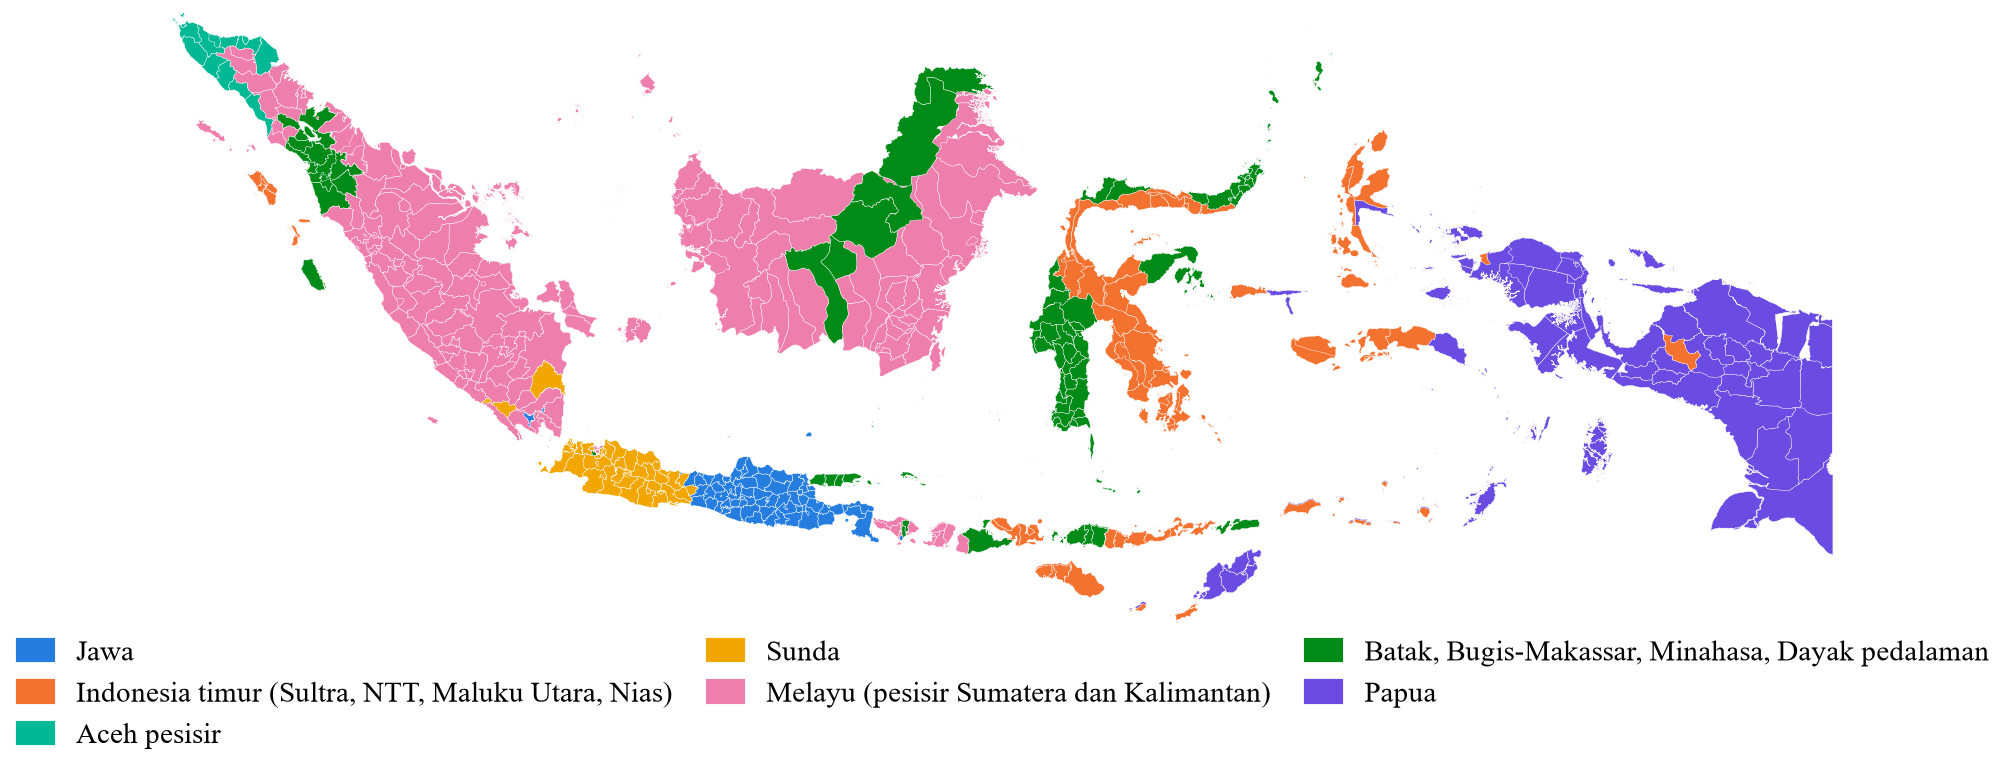
\includegraphics[width=\textwidth]{laporan_klaster.png}
\caption{Klaster kabupaten hasil K-Means ($k = 7$) dari kemiripan nama desa, tanpa label provinsi atau wilayah. Nama klaster diberikan penulis setelah membaca isi setiap klaster.}
\label{fig:klaster}
\end{figure*}

Kesalahan model tidak acak. Pasangan yang paling sering tertukar adalah provinsi bertetangga atau hasil pemekaran dengan budaya yang sama: 29,0\% desa DIY ditebak Jawa Tengah dan 28,1\% desa Banten ditebak Jawa Barat. Di tingkat wilayah (Gbr.~\ref{fig:confusion}), 26\% desa Kalimantan ditebak Sumatera, yang dapat dijelaskan oleh kosakata Melayu yang sama seperti \textit{sungai}, \textit{tanjung}, dan \textit{teluk}.

Temuan paling menarik adalah jejak transmigrasi. Di provinsi tujuan transmigrasi (Lampung, Sumatera Selatan, Jambi, lima provinsi Kalimantan, dan Sulawesi Tengah), 8,4\% desa ditebak sebagai provinsi di Jawa, hampir dua kali lipat provinsi luar Jawa lainnya (4,3\%). Pola ini paling kuat di Lampung (16,3\%), terutama di Kota Metro (45,5\%) dan Kabupaten Pringsewu (33,6\%), yang berada di kawasan kolonisasi awal sejak 1905 \cite{sudarno2018}. Gbr.~\ref{fig:jejak} memetakan pola ini per kabupaten.

Bukti yang tidak bergantung pada model juga ditemukan: 96 desa di luar Jawa memakai nama kabupaten/kota di Jawa sebagai kata utuh, seperti ``Purworejo'', ``Sukoharjo'', ``Klaten'', dan ``Sumbersari Bantul'', dan 41 di antaranya berada di Lampung. Para pendatang menamai desa barunya dengan nama kampung halamannya.

Ada dua catatan. Pertama, Bali juga sering ditebak Jawa (17,9\%), tetapi Bali bukan tujuan transmigrasi; ini lebih tepat dijelaskan oleh kedekatan bahasa dan budaya Jawa dan Bali. Kedua, di Kalimantan dan Sulawesi Tengah angkanya tidak jauh di atas rata-rata. Dugaan penulis, desa transmigrasi yang lebih baru banyak diberi nama berbahasa Indonesia umum seperti ``Karya Jaya'' atau ``Sumber Makmur'', bukan nama Jawa; dugaan ini perlu diuji lebih lanjut.

Kandidat kesalahan kode wilayah hanya berjumlah 62 desa (0,07\%). Setelah diperiksa, sebagian besar adalah nama pendek yang kebetulan mirip pola daerah lain, seperti ``Golo'' dan ``Tumba'', atau nama yang memang dipakai di banyak provinsi. Dengan demikian tidak ditemukan tanda jelas kesalahan kode pada data Kepmendagri 2025.

\subsection{Klastering Kabupaten}

\textit{Silhouette score} tidak memiliki puncak tunggal yang tajam. Nilai tertinggi diperoleh pada $k = 13$ (0,267), tetapi selisihnya dengan $k = 7$ (0,247) kecil, dan semua nilai berada di bawah 0,3. Hal ini menunjukkan bahwa nama desa berubah secara bertahap dari satu daerah ke daerah tetangga, bukan berpindah secara tiba-tiba. Nilai $k = 7$ dipilih karena merupakan puncak lokal pertama untuk kedua metode, masih dapat ditafsirkan satu per satu, dan sama dengan jumlah wilayah besar sehingga dapat dibandingkan langsung. K-Means dipakai sebagai hasil utama karena \textit{silhouette}-nya lebih tinggi (Tabel~\ref{tab:klaster}). Peta hasil Ward dan peta tujuh wilayah resmi sebagai pembanding tersedia di repositori proyek.

\begin{table}[!t]
\caption{Evaluasi klastering kabupaten pada $k = 7$}
\label{tab:klaster}
\centering
\begin{tabular}{lccc}
\toprule
Metode & Silhouette & ARI provinsi & ARI wilayah \\
\midrule
K-Means & \textbf{0,247} & 0,165 & 0,418 \\
Ward & 0,222 & \textbf{0,182} & \textbf{0,456} \\
\bottomrule
\end{tabular}
\end{table}

ARI terhadap wilayah resmi sebesar 0,42 sampai 0,46 berarti klaster jauh lebih mirip pembagian wilayah daripada pengelompokan acak, tetapi tidak identik. Justru perbedaannya yang menarik (Gbr.~\ref{fig:klaster}). Tanpa diberi label apa pun, Pulau Jawa terbelah menjadi klaster Sunda (Jawa Barat dan Banten) dan klaster Jawa (Jawa Tengah, DIY, dan Jawa Timur), mengikuti batas bahasa dan bukan batas pulau. Batas klaster juga memotong batas provinsi mengikuti batas suku: klaster Aceh hanya berisi Aceh pesisir, sementara dataran tinggi Gayo dan Alas masuk klaster lain; Sumatera Utara terbelah menjadi tanah Batak, pesisir Melayu, dan Nias; serta Kota Metro dan Pringsewu di Lampung masuk klaster Jawa, konsisten dengan temuan transmigrasi. Sebagian besar Sumatera dan Kalimantan bergabung dalam satu klaster Melayu. Keterbatasannya, Bali tidak membentuk klaster sendiri dan sebagian besar kabupatennya masuk klaster Melayu.

\subsection{Generator Nama Desa}

Tabel~\ref{tab:orde} menunjukkan pengaruh orde rantai Markov. Orde 2 menghasilkan banyak nama baru tetapi kurang khas, sedangkan orde 4 lebih sering menyalin nama yang sudah ada. Orde 3 dipilih sebagai titik tengah.

\begin{table}[!t]
\caption{Pengaruh orde generator (rata-rata tujuh wilayah)}
\label{tab:orde}
\centering
\begin{tabular}{ccc}
\toprule
Orde & Nama baru (\%) & Dikenali classifier (\%) \\
\midrule
2 & 90,5 & 55,0 \\
3 & 85,5 & 72,3 \\
4 & 69,0 & 74,3 \\
\bottomrule
\end{tabular}
\end{table}

Dari 350 nama karangan (50 per wilayah), 71,7\% ditebak classifier sesuai wilayah asal generatornya, jauh di atas tebakan acak (14,3\%). Contoh hasilnya antara lain ``Cikayung'' dan ``Lebangwetan'' (Jawa), ``Lubuk Simodo'' (Sumatera), ``Lintai Hilir'' (Kalimantan), dan ``Wugunggunome'' (Papua). Angka ini perlu dibaca hati-hati: generator cenderung memakai pola yang paling umum di wilayahnya, sehingga wajar jika nama karangan lebih mudah dikenali daripada nama asli. Hasil ini menunjukkan bahwa ciri nama per daerah cukup kuat untuk ditiru, bukan hanya dikenali.

\subsection{Purwarupa}

Dasbor dapat diakses di \url{https://jejaknama.streamlit.app}. Halaman tebak nama menampilkan tiga provinsi teratas beserta probabilitasnya, peta peluang per provinsi, dan mewarnai huruf-huruf yang paling mendorong tebakan berdasarkan kontribusi koefisien Logistic Regression. Halaman lain menyajikan peta klaster, n-gram khas, peta jejak transmigrasi, generator nama, serta dua kuis untuk presentasi: ``Asli atau Palsu?'' dan ``Manusia vs Mesin''.

\section{Kesimpulan dan Saran}

Penelitian ini menunjukkan bahwa nama desa di Indonesia menyimpan informasi budaya yang dapat diukur. Dari susunan huruf saja, model menebak provinsi dengan akurasi sekitar 40\% dan wilayah besar 65\% sampai 68\%, jauh di atas tebakan acak. N-gram yang paling menentukan sesuai dengan ciri bahasa daerah. Klastering tanpa label menghasilkan pembagian yang mengikuti batas bahasa dan suku, seperti pemisahan Sunda dan Jawa. Kesalahan model pun bermakna, karena memperlihatkan jejak kolonisasi dan transmigrasi di Lampung. Terakhir, pola nama per daerah cukup kuat untuk ditiru oleh generator sederhana.

Beberapa keterbatasan dan saran pengembangan:
\begin{itemize}
\item Provinsi hasil pemekaran yang budayanya sama hampir mustahil dibedakan dari nama saja; untuk aplikasi praktis, tebakan wilayah dan top-3 lebih bermakna.
\item Pemilihan $k$ pada klastering sebagian didasarkan pada pertimbangan praktis. Metode klastering lain seperti model campuran atau klastering hierarkis dengan visualisasi dendrogram dapat dicoba.
\item Aturan asosiasi (Apriori atau FP-Growth) pada kata penyusun nama desa dapat dipakai untuk menemukan pasangan kata yang sering muncul bersama, misalnya ``sido'' dengan ``mulyo''.
\item Pendekatan yang sama dapat diterapkan pada nama tempat di seluruh dunia, misalnya memakai data GeoNames, untuk menebak negara dari nama kota.
\item Model berbasis jaringan saraf tingkat karakter dapat dibandingkan dengan model klasik yang dipakai di sini.
\end{itemize}

\begin{thebibliography}{00}
\bibitem{ambekar2009} A. Ambekar, C. Ward, J. Mohammed, S. Male, and S. Skiena, ``Name-ethnicity classification from open sources,'' in \textit{Proc. 15th ACM SIGKDD Int. Conf. Knowledge Discovery and Data Mining (KDD)}, Paris, France, 2009, pp. 49-58, doi: 10.1145/1557019.1557032.

\bibitem{ye2017} J. Ye, S. Han, Y. Hu, B. Coskun, M. Liu, H. Qin, and S. Skiena, ``Nationality classification using name embeddings,'' in \textit{Proc. 2017 ACM Conf. Information and Knowledge Management (CIKM)}, Singapore, 2017, pp. 1897-1906, doi: 10.1145/3132847.3133008.

\bibitem{fize2021} J. Fize, L. Moncla, and B. Martins, ``Deep learning for toponym resolution: Geocoding based on pairs of toponyms,'' \textit{ISPRS Int. J. Geo-Inf.}, vol. 10, no. 12, p. 818, 2021, doi: 10.3390/ijgi10120818.

\bibitem{cavnar1994} W. B. Cavnar and J. M. Trenkle, ``N-gram-based text categorization,'' in \textit{Proc. 3rd Annu. Symp. Document Analysis and Information Retrieval (SDAIR)}, Las Vegas, NV, USA, 1994, pp. 161-175.

\bibitem{sujaini2024} H. Sujaini and A. B. Putra, ``Analysis of language identification algorithms for regional Indonesian languages,'' \textit{IAES Int. J. Artif. Intell. (IJ-AI)}, vol. 13, no. 2, pp. 1741-1752, 2024, doi: 10.11591/ijai.v13.i2.pp1741-1752.

\bibitem{winata2023} G. I. Winata \textit{et al.}, ``NusaX: Multilingual parallel sentiment dataset for 10 Indonesian local languages,'' in \textit{Proc. 17th Conf. European Chapter of the Association for Computational Linguistics (EACL)}, Dubrovnik, Croatia, 2023, pp. 815-834.

\bibitem{sudarno2018} Sudarno, ``Kebijakan percobaan kolonisasi di Gedong Tataan (Lampung) tahun 1905-1917,'' \textit{Paramita: Historical Studies Journal}, vol. 28, no. 1, pp. 1-12, 2018, doi: 10.15294/paramita.v28i1.10916.

\bibitem{kepmendagri2025} Kementerian Dalam Negeri Republik Indonesia, \textit{Keputusan Menteri Dalam Negeri Nomor 300.2.2-2138 Tahun 2025 tentang Pemberian dan Pemutakhiran Kode, Data Wilayah Administrasi Pemerintahan, dan Pulau}, Jakarta, 2025.

\bibitem{cahyadsn} C. DSN, ``wilayah: Kode dan nama wilayah administrasi Indonesia,'' GitHub repository. [Online]. Available: \url{https://github.com/cahyadsn/wilayah}

\bibitem{salton1988} G. Salton and C. Buckley, ``Term-weighting approaches in automatic text retrieval,'' \textit{Information Processing \& Management}, vol. 24, no. 5, pp. 513-523, 1988.

\bibitem{mccallum1998} A. McCallum and K. Nigam, ``A comparison of event models for naive Bayes text classification,'' in \textit{Proc. AAAI-98 Workshop on Learning for Text Categorization}, 1998, pp. 41-48.

\bibitem{cortes1995} C. Cortes and V. Vapnik, ``Support-vector networks,'' \textit{Machine Learning}, vol. 20, no. 3, pp. 273-297, 1995.

\bibitem{fan2008} R.-E. Fan, K.-W. Chang, C.-J. Hsieh, X.-R. Wang, and C.-J. Lin, ``LIBLINEAR: A library for large linear classification,'' \textit{J. Mach. Learn. Res.}, vol. 9, pp. 1871-1874, 2008.

\bibitem{pedregosa2011} F. Pedregosa \textit{et al.}, ``Scikit-learn: Machine learning in Python,'' \textit{J. Mach. Learn. Res.}, vol. 12, pp. 2825-2830, 2011.

\bibitem{kaufman2012} S. Kaufman, S. Rosset, C. Perlich, and O. Stitelman, ``Leakage in data mining: Formulation, detection, and avoidance,'' \textit{ACM Trans. Knowl. Discov. Data}, vol. 6, no. 4, art. 15, 2012, doi: 10.1145/2382577.2382579.

\bibitem{halko2011} N. Halko, P.-G. Martinsson, and J. A. Tropp, ``Finding structure with randomness: Probabilistic algorithms for constructing approximate matrix decompositions,'' \textit{SIAM Review}, vol. 53, no. 2, pp. 217-288, 2011.

\bibitem{lloyd1982} S. Lloyd, ``Least squares quantization in PCM,'' \textit{IEEE Trans. Inf. Theory}, vol. 28, no. 2, pp. 129-137, 1982.

\bibitem{arthur2007} D. Arthur and S. Vassilvitskii, ``k-means++: The advantages of careful seeding,'' in \textit{Proc. 18th Annu. ACM-SIAM Symp. Discrete Algorithms (SODA)}, 2007, pp. 1027-1035.

\bibitem{ward1963} J. H. Ward, ``Hierarchical grouping to optimize an objective function,'' \textit{J. Amer. Statist. Assoc.}, vol. 58, no. 301, pp. 236-244, 1963.

\bibitem{rousseeuw1987} P. J. Rousseeuw, ``Silhouettes: A graphical aid to the interpretation and validation of cluster analysis,'' \textit{J. Comput. Appl. Math.}, vol. 20, pp. 53-65, 1987.

\bibitem{hubert1985} L. Hubert and P. Arabie, ``Comparing partitions,'' \textit{J. Classification}, vol. 2, no. 1, pp. 193-218, 1985.

\bibitem{shannon1948} C. E. Shannon, ``A mathematical theory of communication,'' \textit{Bell Syst. Tech. J.}, vol. 27, no. 3, pp. 379-423, 1948.

\bibitem{streamlit} Streamlit, ``Streamlit: A faster way to build and share data apps.'' [Online]. Available: \url{https://streamlit.io}
\end{thebibliography}

\end{document}
